\documentclass[]{article}
\usepackage{fullpage}
\usepackage[authoryear]{natbib}
\usepackage{setspace}
    \doublespacing
\usepackage{hyperref}
\hypersetup{
    colorlinks,
    citecolor=black,
    filecolor=black,
    linkcolor=cyan,
    urlcolor=cyan
}
\usepackage{amssymb,amsmath}
\usepackage{bm}
\usepackage{dcolumn}
\usepackage{booktabs}
\usepackage{url}
\usepackage{tikz}
\usepackage{todonotes}
\usepackage[utf8]{inputenc}
\usepackage{graphicx}
\usepackage{longtable}
\usepackage{todonotes}
\usepackage{lscape}
\usepackage{float}

\usepackage[margins]{trackchanges}


\title{Fiscal Rule Stretching in Europe During Financial Market Stress and Crises}

\author{Christopher Gandrud \\ \emph{City University London} \\ \emph{Hertie School of Governance}\footnote{Please contact Christopher Gandrud
(\href{mailto:christopher.gandrud@city.ac.uk}{\nolinkurl{christopher.gandrud@city.ac.uk}}) or Mark Hallerberg (\href{mailto:hallerberg@hertie-school.org}{\nolinkurl{hallerberg@hertie-school.org}}). Thank you to workshop participants at Texas A \& M University. Our research is generously supported by the Deutsche Forschungsgemeinschaft (No. HA5996/2-1). Replication material can be found at: \url{https://github.com/christophergandrud/eurostat_revisions}.}
\and
Mark Hallerberg \\ \emph{Hertie School of Governance}}

\begin{document}

\maketitle

\addeditor{MH}
\addeditor{CG}

\begin{center}
    \textbf{Incomplete working draft. Comments and suggestions very welcome.}
\end{center}

\begin{abstract}
    Elected governments have incentives to stretch accounting rules by classifying loss-making and/or indebted endeavors, such as public companies and pension schemes, as off of the public balance sheet. Doing so improves the appearance of the incumbent government to cost-conscious voters and fiscally important international institutions. We expect rule stretching to be especially prevalent during periods of financial market stress and crisis given the large expense of responding to these events. In addition, policy options available to aid troubled financial institutions, such as liquidity assistance, bad banks, and bank nationalizations, are often hard to classify as being inside or outside of the government sector, thus making it more likely that governments will stretch how they are classified. To test these propositions, we examine revisions to government debt and deficit figures made by the European statistical agency--Eurostat. These revisions frequently occur because this politically independent agency re-classifies member state policies and organisations as being within the government sector, when a national government had originally classified them as outside. We find that debt figures are more likely to be revised upwards for years close to national elections, especially when unscheduled. Such election effects are heightened further by financial market stress. Our research underlines the importance of having a vigilant and strongly politically independent government statistical agency during periods of financial market stress to ensure reliable government finance statistics.
\end{abstract}

\section{Introduction}

This paper examines why governments stretch the rules when they determine how policies impact their debts and deficits, especially during periods of financial market stress and turmoil. By ``rule stretching'' we mean that when the fiscal implications of a policy are potentially ambiguous, a decision is made to minimise how it affects the public balance sheet. This research question affects other literatures in political science in interesting ways. One strand examines the relationship between the reporting of data and the quality of governance \cite[e.g.][]{Hollyer2014}. \cite{Alt2014} explore the relationship among the transparency of fiscal data, elections, and pressure from the European Union. They argue that European Union member states were more likely to violate the Eurostat statistical agency's rules for reporting budget data when fiscal transparency was low and when it was an election year in ways that made the government look better to voters. A related strand focuses on the economic vote and whether or not voters notice or incorporate information about these revisions into their decisions. \cite{KayserLeininger2015} find that the press, and voters as a result, do not pay attention to revised figures.

Our paper builds on insights on data revisions by Kayser and Leininger and on elections and fiscal transparency by Alt, Lassen, and Wehner to explore the implications of their arguments for government action.\todo{Mark: maybe also cite on the international channel?} If voters care most about reported, rather than actual, figures then governments have an incentive to manipulate them before elections. One would expect greater manipulations in ways that make the government's stewardship of the public balance sheet look better as elections approach. There is also an indirect electoral channel that runs through international institutions and investors for some countries. Especially in the European Union where members' budgets are constrained by the Stability and Growth Pact, fiscal rule stretching in one policy area allows governments to not have to cut back as much in others areas voters care about in order to meet internationally agreed commitments. Countries that rely on foreign sovereign bond investors may similarly rule stretch in order to maintain an attractive balance sheet for foreign sovereign bond investors, thus allowing them to fund programs that voters want.

During a financial crisis, governments' electorally motivated fiscal rule-stretching is potentially even more pronounced. Financial crises substantially strain public budgets as economic activity and so tax revenue decrease while bank bailout policies incur significant expenses. At the same time, many tools commonly used to respond to financial crises--guarantees, liquidity assistance, public asset management companies--have potentially ambigious fiscal implications. So, during a financial crisis politicians have even stronger incentives and potentially capabilities to rule-stretch around elections.

We can measure these activities by looking at revisions of budget figures, and in particular debt.

We also explore two main alternative hypotheses. The first alternative focuses on ``shocks'' to the economy, which in turn affect government statistics. Countries with more shocks may engage in more revisions, with the bias depending upon the nature of the shocks (positive or negative). One can expect that the shocks are symmetrical, where the greater the shock the more the potential revision, or that one direction requires more revisions, with  the relative elasticities of taxes making one direction more volatile than another. This would be the standard ``economic'' argument. These revisions, however, should be due to ``economic'' effects and not conscious government manipulation. The forecasting literature in economics includes such measures. The second one considers institutional arguments about who generates the numbers. In some countries, the government does the reporting, while in others an independent body plays this role. Of course, these three arguments may be related in theoretically interesting ways. For example, a country experiencing a positive shock may be more likely to call an election in countries where elections are unscheduled.

Our dataset is composed only of European Union member states. This is useful for several reasons. They face one international organisation that has two sets of rules on economic matters for its members that are often closely related, namely those rules for Member States inside the eurozone and those outside, which are nevertheless the same when it comes to the reporting of the data, though incentives to follow the rules differ. Moreover, there is one body that can provide comparative data that we can analyse. While fiscal figures are initially generated by national agencies, as part of Stability and Growth Pact (SGP) deficit and debt limit enforcement all Member States face one set of accounting rules (the European System of Accounts or ESA) for data they report to the EU and they have one body, Eurostat, that ultimately enforces it. Eurostat regularly revises Member State data so that it conforms to the common rules. This means that differences across countries in initial reporting are not due to different accounting rules, but instead often different interpretations of these rules. Finally, they are all parliamentary or semi-presidential systems where elections are crucial for the formation of governments.

We find that Member State debt figures are more likely to be revised upwards for years close to national elections, especially when these are unscheduled. This suggests that governments are more prone to rule stretch closer to elections. They tend to ``low ball'' how much policies will cost closer to elections thus leading to an upward Eurostat revision in later years. Such election effects are strengthened further by financial market stress. Our research underlines the importance of having a vigilant and politically independent government statistical agency during periods of financial market stress to ensure reliable government finance statistics.\todo{How do we want to handle the deficit findings?}

\section{Political budget cycles and fiscal gimmicks}

The revision of government-reported statistics is of interest for several reasons.

The reporting of statistics, or the lack of it, may tell one about the overall governance of a given country. \cite{Hollyer2014} argue that the lack of reporting is not random. They record the availability of data for 125 countries over a thirty-year period. They analyse this data with Bayesian Item Response model to create a transparency index. They then use this index to predict the quality of governance in autocracies. In other work, they anticipate that this type of transparency affects government accountability, as well as collective action \citep{hollyerforthcoming}.\footnote{\cite{jervin2013} tells a similar story for African countries. The quality of data is generally good when governments have state capacity to provide them. When those governments get into trouble, however, so that their capacity declines the quality of the data also drops.}

While \cite{Hollyer2014} consider how voters might react under conditions when they get data and when they do not, there is a separate literature on the economic vote that assumes that voters have no trouble accessing regular data on the state of the economy and they use this to decide about the competence of the government in managing economic policy. One debate considers whether voters are prospective or retrospective. On the latter, the assumption is that voters observe outcomes, and they decide whether to support the incumbent government. In response to the strong assumptions about voter knowledge, there is a growing literature on ``real-time fiscal policy''. \cite{KayserLeininger2015} argue that the press ignores revisions to data. Moreover, \cite{kayser_peress} find that voters pay particular attention to data they do not experience themselves. They observe unemployment, for example, but they do not observe economic growth and rely on reported figures when making decisions about which party to support. In our case, we are interested in government fiscal data that only the government can report. If one combines the insights in the two papers, they suggest that voters make decisions on the first set of data they see. This would make manipulation of such data potentially rewarding for governments that seek to remain in office.

We build on this insight for our core argument. Following \cite{nordhaus1975} as well as \cite{Alt2014}, one would anticipate that there are opportunistic business cycles where governments manipulate macro-economic tools at their disposal in an effort to make the economy look better before an election. \cite{clark2003} finds the tools a government uses depends upon the logic of the Mundell-Fleming model: if one assumes that capital is mobile, a government relies on monetary policy when the exchange rate is flexible while it leans on fiscal policy when the exchange rate is fixed. Both Nordhaus and Clark, however, focus on actual economic output from the use of these instruments. We are interested in the perceived figures prior to an election. There is a possible spin-off on the Clark argument. One can expect that extra spending in EU member states with flexible exchange rates has no macro-economic payoffs, while it does have payoffs in countries with fixed exchange rates, which will mostly be those in the eurozone.\footnote{Exceptions would be those countries that fix their exchange rate to the euro or that have very narrow bands. Some central and East European countries like Lithuania, for example, have (or had) currency boards that maintained a de facto fix. Denmark has chosen not to join the eurozone, but it maintains a tight band around the euro for its kronor.} Governments may, however, want to look good to their voters on these figures even in the flexible exchange rate countries in the dataset. This suggests that there should be cycles in revisions to figures according to elections, but that the revisions should be in all member states. \cite{DeCastro2013} in fact find using pre-crisis data that fiscal data for years closer to elections are revised by Eurostat more.

Moreover, we add two additional parts to the model. First, and separate from \cite{Alt2014} who focus on all election years, we anticipate that manipulation of figures is greater when the government calls the election--i.e. it is unscheduled--instead of allowing it to go to full term. The reason follows the insights of \cite{clark2003} on the use of instruments, but with the expectation that elections called quickly--largely for non-fiscal or economic reasons--do not give the government time to affect the economy directly either through monetary or fiscal policy. \cite{Kayser2005} finds that manipulation of the economy before unscheduled elections is too cumbersome and too difficult to time. This suggests that the manipulations are substitutes for actual instrument use.

Second, we are interested in circumstances under which governments more easily can manipulate the figures. Where are the ``grey'' areas in terms of the classification of assets and liabilities? For \cite{Alt2014}, those ``grey'' areas are in the budgetary shadows, in places where there is less transparency. We focus on specific types of operations in this paper. In particular, Eurostat has been active clarifying initially ambiguous rules on how to treat assistance to the financial sector \cite[see][]{GandrudHallerberg2016}. There is a potential endogeneity problem to using actual operations, however; ultimately, a government decides which tools to use, as \cite{GandrudHallerberg2016} explore in more detail. As we explain below, we measure overall financial market stress instead of actual realisations, which are part of what the government is manipulating in the first place.

Domestic voters, however, may not be the actors the government is directly trying to impress with its budget statistics. There is evidence that countries intentionally distort statistics so that they receive some sort of payoff from an international organisation. For example, \cite{kerner2016} find that some African countries kept their per capita incomes below the eligibility threshold for World Bank’s International Development Association (IDA). This is a clear case where governments change their official statistics in response to an expectation from an international organisation.

Reported outcomes in terms of economic and fiscal data have a real impact on policy especially in European Union countries because of the role of the European institutions, and in particular the European Commission and Council of Ministers. GDP figures affect what type of co-financing governments receive from the European Union for a range of activities, such as environmental protection, guarantees for loans that Small and Medium-sized Enterprises (SMEs) take, and the construction of roads.\footnote{The amounts can be substantial as a percentage of total funding for a given project, up to 85 percent of the cost of the project in regions judged to be “Less Developed”, which are those with a per capita income below 75 percent of the European Union average.} Under the Stability and Growth Pact, all Member States are expected to have budget balances no worse than 3 percent of GDP and debt burden no greater than 60 percent of GDP. The European Commission decides each year whether a member state has an ``excessive deficit'', with those earning this distinction under the Commission subject to an Excessive Deficit Procedure (EDP). Member states must propose corrective methods. The subset that are also eurozone members face potential penalties, such as fines. Member states that do not adjust their performance also could lose their access to structural and cohesion funds, which are the largest part of the European Union budget.

There are two alternative hypotheses that are relevant here. One could ask whether countries that have clear biases concerning future performance have similar biases concerning current performance. This means looking at the literature on forecasting, which  considers why there are biases in forecasting numbers. Some governments seem to be eternal optimists; they report figures that that always appear to be better than turn out to be. Others are chronic pessimists, and they have positive ``surprises''. Looking at European Union member states, work from the early years of the euro finds that some types of spending are procyclical, such as public investment spending. There is also a pronounced electoral cycle in the forecasting literature, with more optimistic forecasts for electoral years \citep{hallerbergstrauch2002}. This work, and others like it, usually consider the size of the ``shock'' that a country experiences, both in terms of the magnitude (usually by taking the absolute value of the deviation) and the direction of the shock. In more recent work, \cite{hallerbergstrauch209} find that European Union member states that fit most closely a ``fiscal contracts'' approach to budgeting have more conservative forecasts than member states that fit better a ``delegation to a strong finance minister'' approach.

This discussion leads us to as second possible alternative explanation to explore, namely an  institutional one. \emph{[undeveloped]  The predictions, however, are not so clean. One can imagine that if there are fiscal contracts in a country like the Netherlands, one might fudge numbers so the you more or less comply with internal targets. If it turns out later the government missed the target, this is unlikely to bring down the government. At the same time, precisely because  there is a temptation to do this one might have especially competent staff do the numbers. The Dutch largely outsource the production of the figures to the CPB, which, while technically part of the executive, has established a reputation since the end of World War II as an independent body. What may ultimately matter most, then, is the relative independence of the body that reports the data. Delegation to a strong finance minister may suggest that the finance ministry does the numbers. This, too, can be checked, as happened in the United Kingdom, when frustration with habitually optimistic figures led to pressure for an objective body, which was the inspiration for the Office of Budget Responsibility created in 2010. How to measure the independence of the statistical agency, however, is not straight-forward.}

\section{Rule stretching during financial crises}

Governments in countries that experience financial market stress and crises face considerable fiscal difficulties \cite[see][]{Laeven2012} that heighten politicians' incentives to rule stretch. At the same time, and an unexplored area in the literature, the policy options available to politicians to respond to financial crises--e.g. buying equity in a failing bank, bad banks, and bank nationalisations--present numerous rule stretching opportunities. As such, we expect politicians to engage in rule stretching even more during periods of financial market stress and crisis.

\cite{GandrudHallerberg2016} argue that many of the policies available to politicians, especially during the 2008-2011 crisis in Europe were both rarely used previously and had potentially ambiguous debt and deficit implications. For example, if a government buys equity in a troubled bank as, for example, Ireland did with Irish Nationwide Building Society and the Educational Building Society in 2010 has the government spent money or does it have a different, but equivalently valued asset? Does the transaction increase the deficit, or is it what European System of Accounts (ESA 95)--the common European fiscal accounting rulebook at the time--termed a ``financial transaction'', with no effect on the deficit? If a government owns a stake in an asset management company (AMC) used to clean up a failed bank, as the German government did with its AMCs, are the AMC's liabilities government liabilities counted against its debt? Or are they what the ESA 95 terms ``contingent liabilities'', where the government is liable only if the AMC cannot repay them?

Given strong incentives for governments to minimise debt and deficit increases around elections and especially during crises, they have strong incentives to  classify initially such policies in the best possible light, so as not to increase public debts and deficits. In other words, politicians have strong \emph{incentives} and many \emph{opportunities} to fiscal rule stretch during periods of financial market stress.

\section{Hypotheses}

We test the following hypotheses regarding fiscal rule stretching--as measured by Eurostat revisions to member states' debt and deficit figures--around elections and during financial market stress:

\begin{quote}
    $H_{1}$: Debt revisions will be larger for years closer to national government elections.
\end{quote}

\begin{quote}
    $H_{2}$: Debt revisions will be greater for years when there are unscheduled elections.
\end{quote}

\begin{quote}
    $H_{3}$: The effects predicted by $H_{1}$ and $H_{2}$ will be stronger when a country also has high financial market stress.
\end{quote}

\todo[inline]{Deficit hypotheses?}

\section{Empirical tests: Set up}

To test our hypotheses, we ran a series of linear regressions with cumulative debt revisions made by Eurostat as the dependent variable and a number of relevant political and economic indicators on the right-hand side. Because cumulative debt revisions are autoregressive, we also include lagged cumulative debt revisions on the right-hand side in all models.

\subsection{Dependent variable: Eurostat revisions}

We gathered a data set of all revisions that Eurostat made to EU member state debt figures from 2003 through 2013.\footnote{PDF files with the fiscal figures were downloaded from \url{http://ec.europa.eu/eurostat/news/news-releases}. Accessed March 2015.} This sample includes at least three years of data which Eurostat revised for all current (as of 2016) EU member states. Eurostat publishes revisions bi-annually--typically once at the end of April and again in late October. These revisions cover government finance statistics released within the previous four years. As such, the unit of analysis in the following regressions is each Eurostat debt data revision. For every year that government statistics are revised, there are up to seven revisions: The first revision occurs in October of the initial reporting year and continues bi-annually for three years thereafter.

We created a variable of \emph{cumulative revisions for debts} as a percent of GDP up to and including each revision point. We used this as our dependent variables. For cumulative debt revisions, the variable ranged from -1.1 to 12.7 percent of GDP.\footnote{For completeness, we did the same for for deficit revisions. For cumulative deficit revisions, the variable ranged from -4.5 to 1.1 percent of GDP. Results from models with deficit revisions are in the Appendix.} It is important to note that all of these revisions were not due to updates made to the denominator, or to GDP. Eurostat reports GDP revisions separately from corrections made to debt figures. As \cite{DeCastro2013} found for similar Eurostat data in a shorter pre-financial crisis sample, there is a clear tendency for debt statistics to be revised upward, indicating that policies are more expensive than initially reported.

\begin{figure}
    \begin{center}
        \caption{Median \textbf{Debt} Revisions for Data Released Under Various Electoral Conditions}
        \label{median_debt_revisions}
        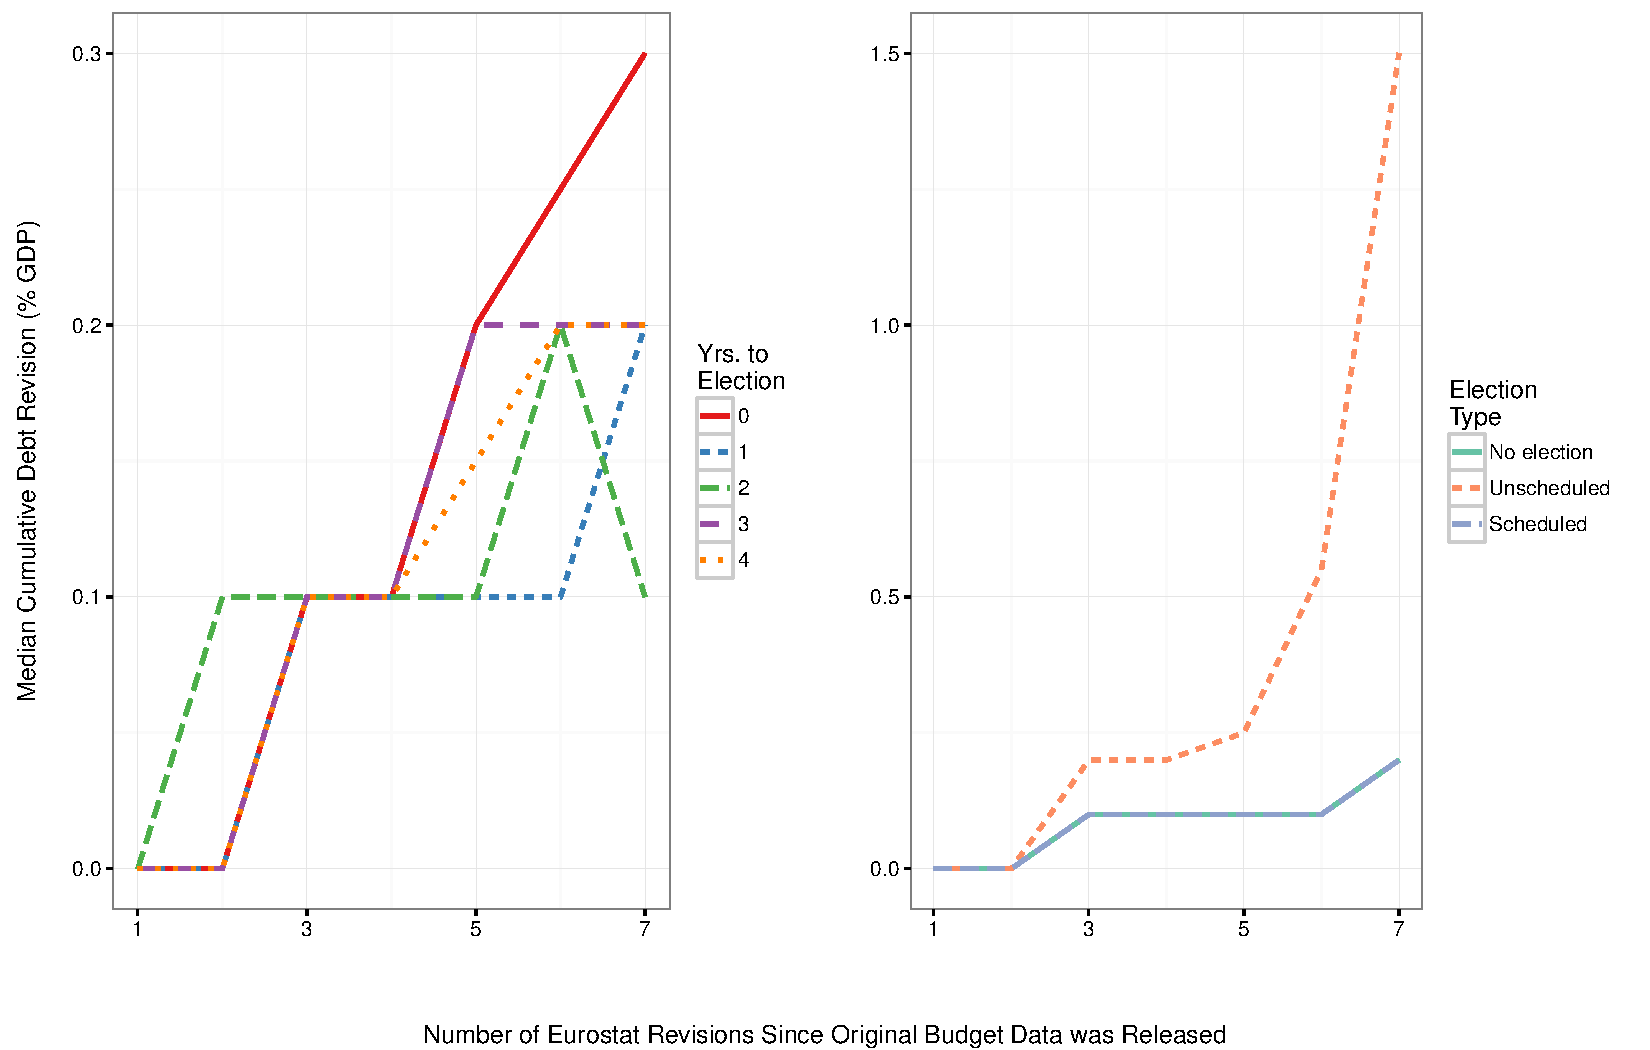
\includegraphics[scale=0.55]{figures/median_debt_revisions.pdf}
    \end{center}
\end{figure}

Figure \ref{median_debt_revisions} shows the cumulative Eurostat debt revisions in our sample under different electoral conditions. Note: below we discuss the electoral variables in detail.\footnote{In figures \ref{median_debt_revisions} and \ref{median_deficit_revisions} we use the original electoral timing variable, not the reversed scale as, in this case, the original scale is easier to interpret.} The left-panel in Figure \ref{median_debt_revisions} clearly indicate that revisions are higher for budget data released in years with elections. Cumulative revisions are similar regardless of election timing until the fifth revision. Over the next two revisions, the median cumulative revision for non-election years remains between 0.1 and 0.2 percent of GDP. In contrast, debt revisions for election years increase to 0.3 percent of GDP by the seventh revision. In the right-panel we can see that the median revision for debt data released for years with unscheduled elections is much higher by the seventh revision (about 1.5 percent of GDP) than for years with scheduled elections or no elections (both are about 0.2 percent of GPD). Again, the divergence in the magnitude of the data revisions largely begins from the fifth revision. These descriptive findings are indications that politicians may indeed be engaging in fiscal rule stretching in election years, especially if they have impromptu elections.

\subsection{Right-hand variables}

To further explore whether governments are more likely to stretch the rules closer to elections and whether this effect interacts with financial market stress, we first use Gandrud's \citeyearpar{gandrudYrcurnt} \emph{years to election} variable in the following regressions. The variable counts down from the year that is the furthest away from the next scheduled election. Election years are recorded as zero, regardless of whether they were scheduled or not. To make the marginal effect estimates from the following regressions more intuitive--i.e. so that a positive coefficient indicates that being closer to an election is associated with an increase in debt data revisions, we reversed the scale election timing scale.\footnote{I.e. for each observed election timing value $x$ for country $i$ and year $t$: $\mathrm{Max}(\mathrm{X}) - x_{i,t}$.}

Not only do we expect that governments are more likely to use rule stretching as elections approach, but that rule stretching should be more prevalent when governments are not able to choose when the election occurs so as to present themselves in the best fiscal light to voters, as well as international institutions and investors that they need to maintain policies that are popular with voters. As such, we also include a categorical variable indicating \emph{election type}. It codes country-years as having a scheduled election, unscheduled election, or no election. The variable is based on \cite{Brender2008}, which was updated and corrected by \cite{hallerbergWehner2015}. Based on our theoretical framework and what we saw in the descriptive statistics, we expect that the revisions will be greater for years when there is an unscheduled election.

To examine how responding to financial market stress may exacerbate governments' fiscal accounting rule stretching behavior, we included Duprey et al.'s \citeyearpar{ThibautDuprey2015} measure of financial market stress. Political economy research has tended to rely on dichotomous financial crisis measures from \cite{Laeven2012} and \cite{ReinhartRog2010} that were \emph{post hoc} hand coded. Problems with these measures are well known \citep[see][]{finstress_paper}. Duprey et al.'s measure has the advantage of being continuous, monthly, and based on a clearly reproducible methodology. They found their indicator for 27 EU member states by measuring co-movements in key financial market characteristics such as equity, bond market, and foreign exchange volatility. The financial market stress variable is able to vary between zero and one, with higher values indicating more financial market stress. To make this monthly measure comparable with our other variables, we found yearly averages. In the sample the variable varies between 0.02 and 0.57.

We hypothesize that the effect of election timing on rule stretching will increase at higher levels of financial market stress. So in the following discussion we focus on interactions between FinStress and the election timing and election type variables.

So far we have only operationalised the direct domestic--voter--audience for rule stretching. To examine the ``international'' audience, we examine whether the level of government gross debts effects the propensity of rule stretching and therefore revisions by Eurostat. Perhaps countries that have higher debts and so are in threat of, or have actually breached, the SGP's limits will be more likely to rule stretch. We would expect that countries in the Eurozone specifically would be more likely to rule stretch when their debts are around and above 60 percent of GDP in order to stay under the SGP's 60 percent debt to GDP limit. A such, we interact central government gross debt

\todo{Rewrite the following paragraph}

If this were the case, we would expect that in our sample, higher deficits will be more strongly associated with revisions than debts. This is because the 3 percent of GDP deficit limit was the focus of EDP enforcement much more so than the 60 percent of GDP debt limit until the advent of the eurozone debt crisis. To test this we gathered general government deficits as a percentage of GDP from Eurostat.\footnote{Available at: \url{http://ec.europa.eu/eurostat/}. Accessed December 2015.} For gross debts, we use information reported by the World Bank's Development Indicators.\footnote{Available at: \url{http://data.worldbank.org/data-catalog/world-development-indicators}. Accessed December 2015.} Both sets of numbers were updated by 2015. \emph{Note that in a future version of the paper we can include a dummy for member states facing an ``excessive deficit procedure'', which only the European Commission may abrogate once that Council of Ministers (ECOFIN) has agreed that a member state indeed has an excessive deficit.}

In some model specifications we included a dummy variable for eurozone membership. An important consideration in enforcement through the EDP is governments' good faith in returning to compliance. Fiscal rule stretching may be viewed as a bad faith move. As such countries subject to SGP enforcement may be less likely to rule stretch. All member states are covered under the monitoring procedures of the Stability and Growth Pact. However, non-eurozone members, such as the United Kingdom, face weaker or non-existent enforcement actions if they breach the SGP's debt and deficit limits. As such, we would expect that higher revisions would be associated with being outside of the eurozone. Conversely, inspired by \cite{clark2003}, perhaps countries in the eurozone having fixed exchange rates need to rely more on rule stretching and so eurozone membership is positively associated with revisions. Because of these conflicting predictions, we do not have strong priors on eurozone membership's effect.

It could be that governments subject to higher \emph{fiscal policy transparency} may be less able to engage in fiscal rule stretching as this behaviour could perhaps be noticed earlier. There are reasons to be skeptical of this reasoning. Primarily, rule stretching is often involves the interpretation of highly technical rules that voters likely do not know or have a view on. Regardless, this is an empirical question we address by using a new fiscal transparency index created by \cite{Wang2015}. They measure the degree to which and what type of fiscal data is reported to the International Monetary Fund from 2003 to 2013. Their index ranges can range from zero to 100 (the maximum possible extent) in our sample of EU member states. Fiscal transparency was never statistically significant in any of our models. As such, below we do not show results from models with fiscal transparency included.

Finally, we also examined if economic growth as measured by year-over-year GDP growth (percentage) would affect revisions.\footnote{From the World Bank Development Indicators. Indicator ID NY.GDP.MKTP.KD.ZG. Accessed February 2016.} Perhaps governments with shrinking economies have incentives to rule stretch more \citep{DeCastro2013}. However, the estimated coefficient for this variable was not statistically significant at conventional levels, including in interaction with the electoral variables,\footnote{An interaction between GDP growth and election type was barely significant at the 10 percent level. However, this appears to largely be because GDP declines are associated with financial market stress. Estimates from a financial market stress interaction were much stronger.} so we do not include it in the results below.

\section{Empirical Tests: results}

Table \ref{debt_results} shows our results from linear regressions with cumulative debt and deficit revisions as the dependent variables, respectively. All models include country fixed effects to help account for unobserved country variation. Because a number of the variables are logically highly correlated with each other (e.g. countries under an EDP have high debts), we ran our models in a step-wise fashion.

There appears to be some evidence (at the 10\% level) that the electoral conditions have the hypothesized effect on debt revisions. We estimate (in models 1 and 2, Table \ref{debt_results}) that being closer to elections and having an unscheduled election is associated with larger cumulative Eurostat debt data revisions later on. The election finding somewhat similar in direction and magnitude to what \cite{DeCastro2013} previously uncovered in Eurostat deficit revision data for 15 EU member states in a time-span that largely did not include the Eurozone and related crises.\footnote{Interestingly, we were not able to replicate their electoral effect on deficit findings in our sample. See the Appendix.}

How does financial market stress impact these electoral effects? We hypothesised that they should be stronger at higher levels of stress. Interactive coefficient estimates are in models 5 and 6 of \ref{debt_results}. Rather than trying to divine the substantive implications of these point estimates, we created marginal effect plots and present them in Figure \ref{me_finstress_elect}.

In the left-panel of Figure \ref{me_finstress_elect} we can see the marginal effect of moving a year closer to an election at increasing levels of financial market stress. From this plot, we estimate that at low levels of stress, there is no statistically significant effect of moving a year closer to an election on cumulative debt revisions. However, at higher levels of stress, e.g. above 0.4 (for context, the United Kingdom and Greece during the heights of their crises had financial market stress scores somewhat above 0.4), moving a year closer to an election is associated with a 0.15 percent of GDP upward revision revision to the government's debt data by Eurostat. In the right-panel of Figure \ref{me_finstress_elect} we see a similar estimated effect for having an unscheduled election--rather than a scheduled election or no election--at high levels of financial market stress.

Of the other variables we examined only the level of central government debt was (weakly at the 10\% level) associated with debt revisions. The direction of the effect was as expected: countries with higher debt levels were more likely to have debt data that Eurostat later revised upwards. Governments' with high debts appear to be more likely to engage in fiscal rule stretching. This is likely because they have increased incentives--from voters, the EU, and sovereign bond investors--to decrease or at least slow the increase in their debts.

There does not appear to be a difference between Eurozone members and non-members in terms of how Eurostat revises their debt data. The reasons for this is somewhat inconclusive as there are multiple channels through with governments can be incentivised to rule stretch, only one of which is to stay below Stability and Growth Pact debt rules.

%To get a sense of how these average effects may play out in each country, we predicted the debt revisions by the third revision year for 27 EU member states.\footnote{We did not include the newest member--Croatia--as its figures have been subject to Eurostat oversight for relatively few years.} Using estimates shown in model 9 of Table \ref{debt_results}, we predicted revisions for non-election years, unscheduled election years, and scheduled election years at observed country minimum and maximum FinStress values. The predictions are shown in Figure \ref{country_predict_debt_required}. Please note that while we used observed country FinStress ranges these plots make frequent out of sample predictions as most countries did not have unscheduled and scheduled elections at these levels of stress. Basic country effects correspond to our priors, namely Greece has very large revisions regardless of election year and type. Typically, when countries are fitted to have unscheduled elections at high stress levels, e.g. Belgium, Denmark, Latvia, Ireland, Spain, and so on, we predict that their debt figures will be revised by about 3.25 percentage points of GDP.

%\subsection{Deficit Revisions}

%We also examined if election type and election timing affected the need for revisions to governments' deficit figures (Table \ref{deficit_results}). First, it is interesting to note that while higher debt levels did not appear to be related to debt figures that required more revisions, higher deficit levels are associated with higher deficit revisions. Perhaps this is related to the primary importance of the 3 percent deficit target placed by Stability and Growth Pact monitors for most of the sample until the Eurozone debt crisis.\footnote{Remember that the sample used in our regressions goes through 2011, only one year after the real start of the debt crisis.} Similarly, we find that being in the eurozone decreases the estimated size of deficit, but not debt revisions. Perhaps this is because countries in the eurozone, which are subject to SGP enforcement, were under greater scrutiny and penalty for breaching the SGP's deficit limits. This suggests that having a relatively strong fiscal monitor could decrease governments' tendency to manipulate figures in fixed exchange rate regimes.

%Let's move onto the electoral and financial market stress variables. There does not appear to be an interactive relationship between financial market stress and years to election on deficit revisions. This could be because responses to financial market stress--bank nationalizations, guarantees, and so on--predominantly impact government debts rather than deficits and so opportunities for rule stretching are opportunities for debt rule stretching specifically. There does appear to be a statistically significant relationship between scheduled elections and FinStress that is similar to the interaction between unscheduled elections and stress in the debt revisions models (see Figure \ref{me_finstress_non_endog_deficit} for the marginal effects). More work is needed to understand this finding.

\begin{figure}
    \caption{Marginal Effects of Election Conditions at Various Levels of Financial Market Stress on \textbf{Debt} Revisions}
    \label{me_finstress_elect}

    \begin{center}
        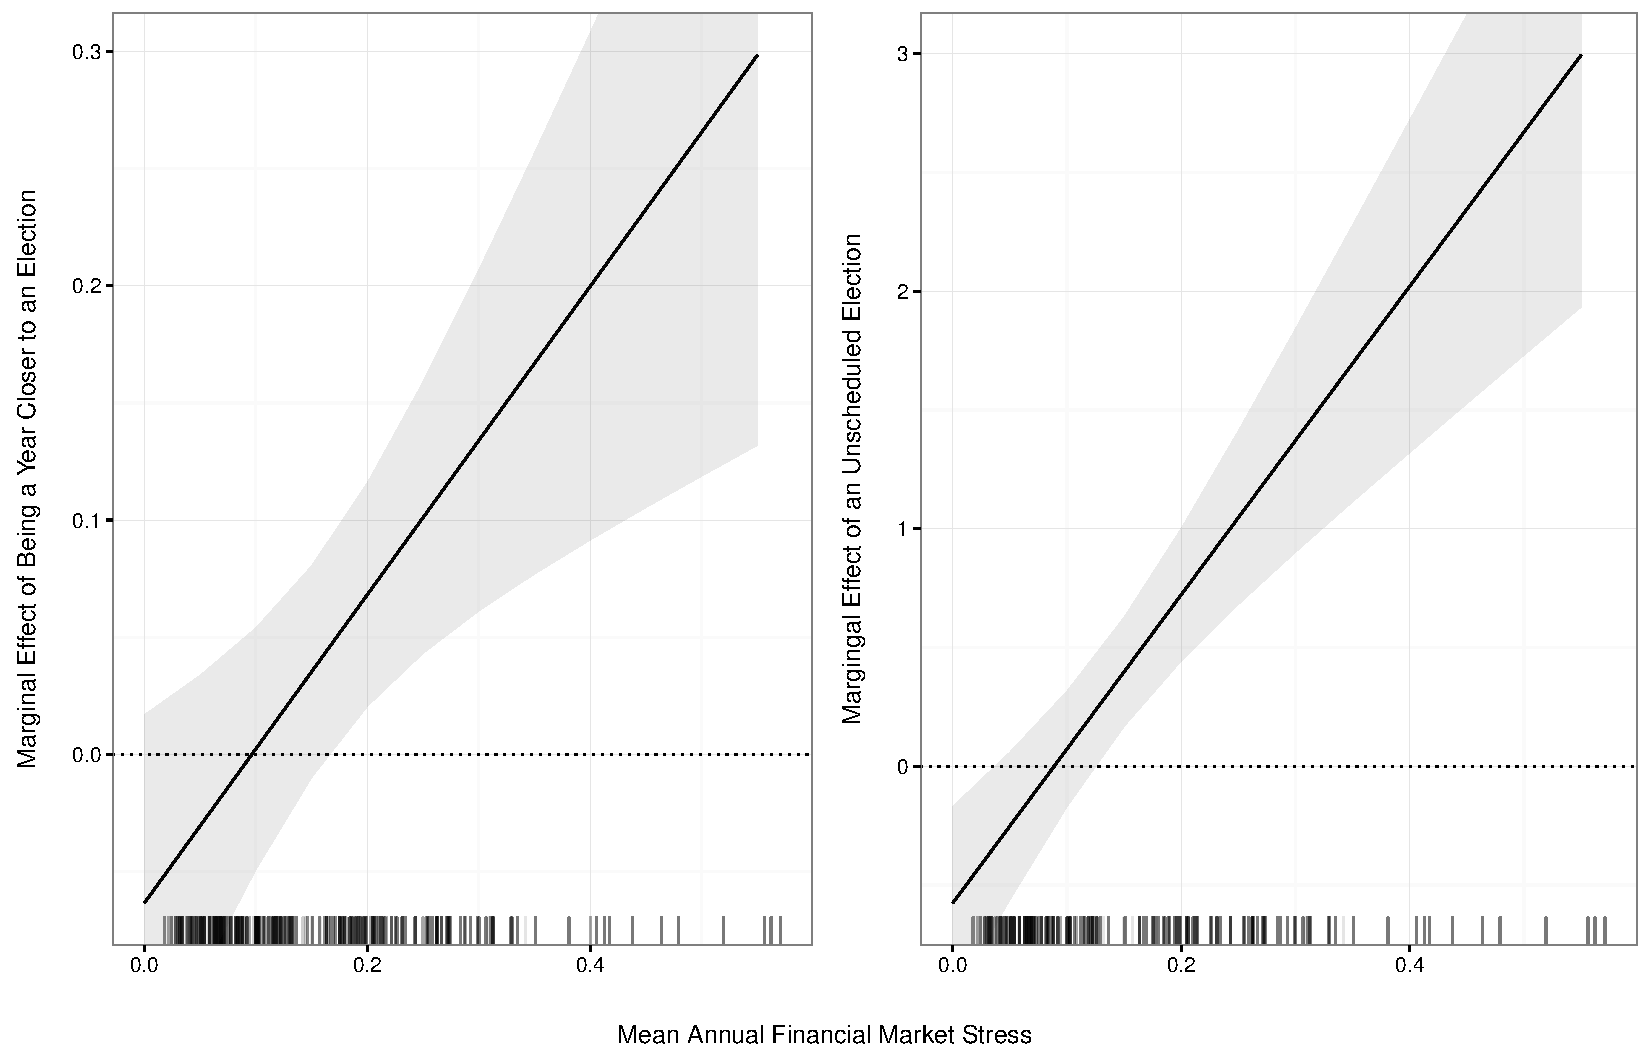
\includegraphics[scale=0.45]{figures/fsi_elect_me.pdf}
    \end{center}

	{\scriptsize{Shaded area represents 95\% confidence interval.}}

\end{figure}

\begin{figure}
    \caption{Marginal Effects of Eurozone Membership and Being in an EDP at Various Levels of Government Debt and Years to Election on \textbf{Debt} Revisions}
    \label{me_debt_edp_elect}

    \begin{center}
        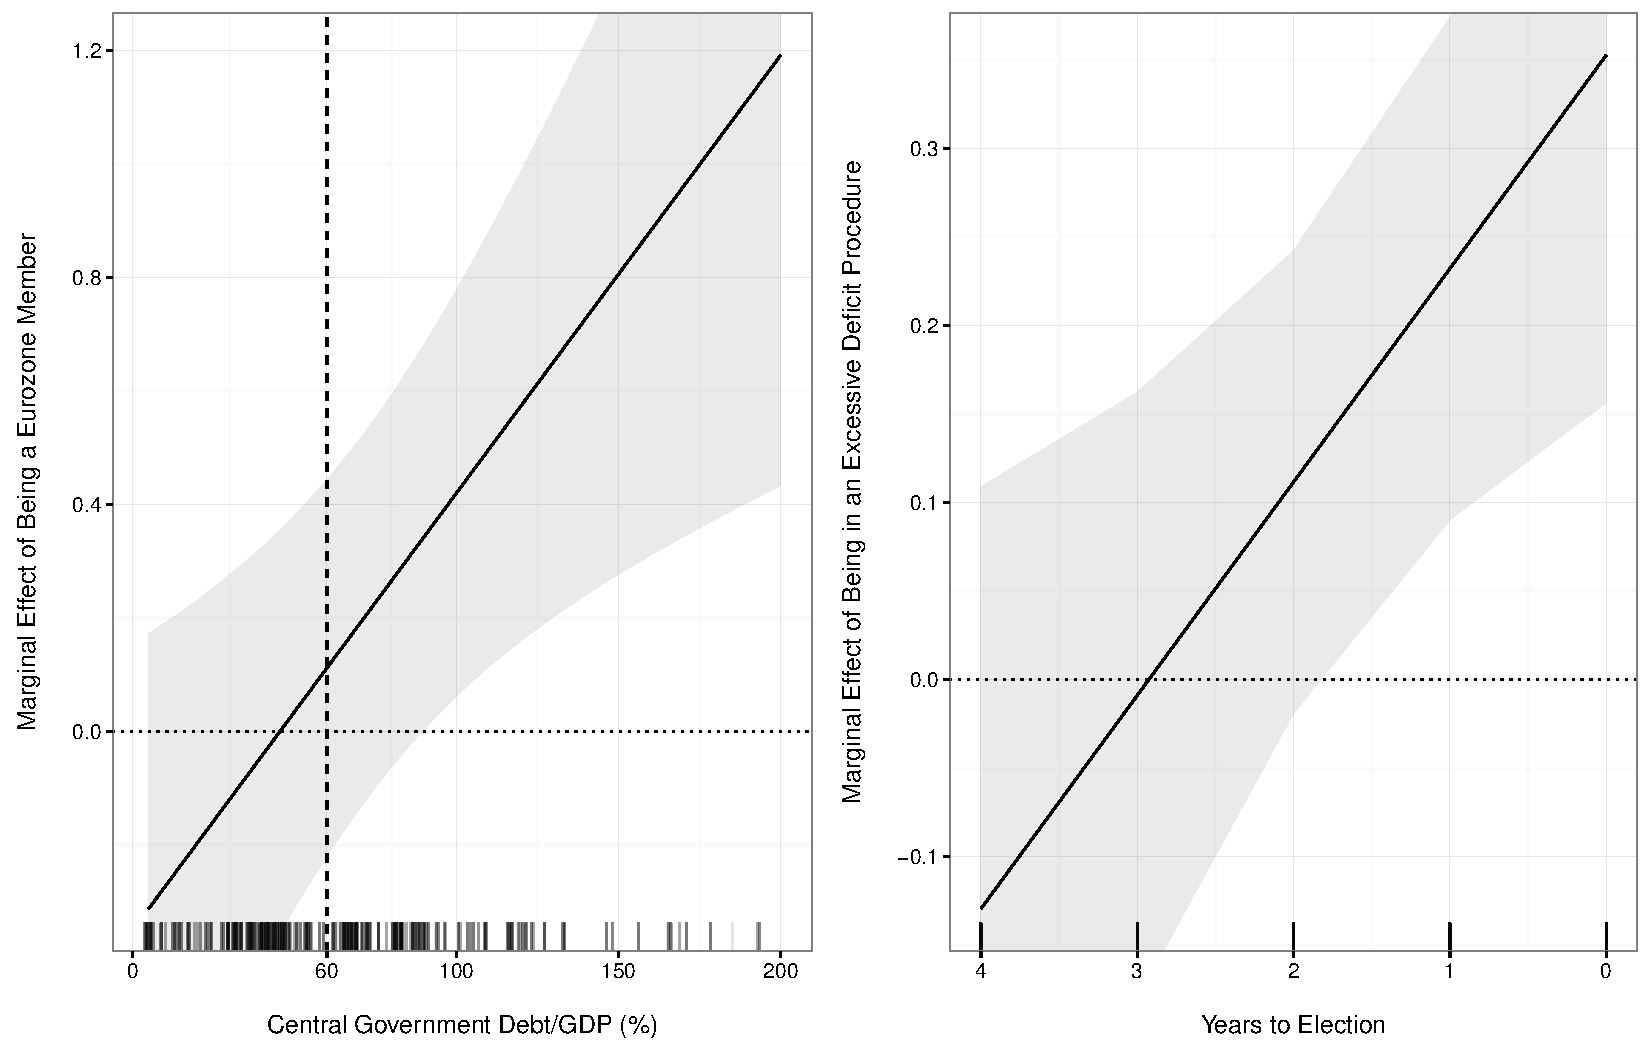
\includegraphics[scale=0.45]{figures/edp_debt_elect_me.pdf}
    \end{center}

	{\scriptsize{Shaded area represents 95\% confidence interval.\\
    The dashed vertical line in the left-panel indicates a debt level of 60\% of GDP. This is the Stability and Growth Pact debt limit past which member states can be put into an Excessive Deficit Procedure.}}

\end{figure}

\begin{landscape}
    
% Table created by stargazer v.5.2 by Marek Hlavac, Harvard University. E-mail: hlavac at fas.harvard.edu
% Date and time: Fri, Feb 12, 2016 - 14:39:59
\begin{table}[!htbp] \centering 
  \caption{Linear Regression Estimation of \textbf{Debt} Revisions} 
  \label{debt_results} 
\tiny 
\begin{tabular}{@{\extracolsep{5pt}}lccccccccccc} 
\\[-1.8ex]\hline 
\hline \\[-1.8ex] 
 & \multicolumn{11}{c}{\textit{Dependent variable:}} \\ 
\cline{2-12} 
\\[-1.8ex] & \multicolumn{11}{c}{Cumulative Debt Revisions} \\ 
\\[-1.8ex] & (1) & (2) & (3) & (4) & (5) & (6) & (7) & (8) & (9) & (10) & (11)\\ 
\hline \\[-1.8ex] 
 Cum. Revisions (lag) & 0.628$^{***}$ & 0.757$^{***}$ & 0.626$^{***}$ & 0.731$^{***}$ & 0.554$^{***}$ & 0.536$^{***}$ & 0.641$^{***}$ & 0.640$^{***}$ & 0.634$^{***}$ & 0.681$^{***}$ & 0.634$^{***}$ \\ 
  & (0.021) & (0.021) & (0.021) & (0.022) & (0.026) & (0.026) & (0.021) & (0.021) & (0.022) & (0.025) & (0.022) \\ 
  & & & & & & & & & & & \\ 
 Election Timing & 0.047$^{*}$ &  & $-$0.031 &  &  &  &  &  & $-$0.064 &  & $-$0.028 \\ 
  & (0.027) &  & (0.047) &  &  &  &  &  & (0.049) &  & (0.040) \\ 
  & & & & & & & & & & & \\ 
 Unscheduled Elect. &  & 0.229$^{*}$ &  & $-$0.560$^{**}$ &  &  &  &  &  & $-$0.576$^{**}$ &  \\ 
  &  & (0.132) &  & (0.235) &  &  &  &  &  & (0.248) &  \\ 
  & & & & & & & & & & & \\ 
 Scheduled Elect. &  & $-$0.001 &  & $-$0.057 &  &  &  &  &  & $-$0.157 &  \\ 
  &  & (0.073) &  & (0.128) &  &  &  &  &  & (0.150) &  \\ 
  & & & & & & & & & & & \\ 
 Financial Stress & 0.039 & 0.191 & $-$1.082$^{*}$ & $-$0.049 &  &  &  &  & $-$1.380$^{**}$ & $-$0.001 & 0.075 \\ 
  & (0.327) & (0.257) & (0.643) & (0.278) &  &  &  &  & (0.651) & (0.331) & (0.343) \\ 
  & & & & & & & & & & & \\ 
 Gen. Gov. Deficit &  &  &  &  & $-$0.004 & 0.010 &  &  &  &  &  \\ 
  &  &  &  &  & (0.011) & (0.011) &  &  &  &  &  \\ 
  & & & & & & & & & & & \\ 
 Cent. Gov. Debt &  &  &  &  & 0.004$^{*}$ & 0.004$^{*}$ &  &  &  &  &  \\ 
  &  &  &  &  & (0.002) & (0.002) &  &  &  &  &  \\ 
  & & & & & & & & & & & \\ 
 Euro Member &  &  &  &  & 0.233 & $-$0.479$^{*}$ & $-$0.006 & $-$0.066 &  &  &  \\ 
  &  &  &  &  & (0.183) & (0.272) & (0.194) & (0.201) &  &  &  \\ 
  & & & & & & & & & & & \\ 
 EDP &  &  &  &  &  &  & 0.163$^{**}$ & 0.041 & 0.175$^{**}$ & 0.083 & $-$0.145 \\ 
  &  &  &  &  &  &  & (0.080) & (0.131) & (0.082) & (0.081) & (0.155) \\ 
  & & & & & & & & & & & \\ 
 Elect. Timing*Fin. Stress &  &  & 0.506$^{**}$ &  &  &  &  &  & 0.658$^{***}$ &  &  \\ 
  &  &  & (0.250) &  &  &  &  &  & (0.252) &  &  \\ 
  & & & & & & & & & & & \\ 
 Unscheduled.Elect*Fin. Stress &  &  &  & 5.818$^{***}$ &  &  &  &  &  & 6.493$^{***}$ &  \\ 
  &  &  &  & (1.443) &  &  &  &  &  & (1.524) &  \\ 
  & & & & & & & & & & & \\ 
 Scheduled.Elect*Fin. Stress &  &  &  & 0.384 &  &  &  &  &  & 0.980 &  \\ 
  &  &  &  & (0.731) &  &  &  &  &  & (0.815) &  \\ 
  & & & & & & & & & & & \\ 
 Cent. Gov. Debt*Euro &  &  &  &  &  & 0.011$^{***}$ &  &  &  &  &  \\ 
  &  &  &  &  &  & (0.003) &  &  &  &  &  \\ 
  & & & & & & & & & & & \\ 
 EDP*Euro &  &  &  &  &  &  &  & 0.191 &  &  &  \\ 
  &  &  &  &  &  &  &  & (0.162) &  &  &  \\ 
  & & & & & & & & & & & \\ 
 Elect. Timing*EDP &  &  &  &  &  &  &  &  &  &  & 0.137$^{**}$ \\ 
  &  &  &  &  &  &  &  &  &  &  & (0.057) \\ 
  & & & & & & & & & & & \\ 
 Constant & 0.648$^{***}$ & 0.361$^{**}$ & 0.831$^{***}$ & 0.353$^{**}$ & 0.251 & 0.316 & 0.658$^{**}$ & 0.688$^{***}$ & 0.807$^{***}$ & 0.343$^{**}$ & 0.752$^{***}$ \\ 
  & (0.188) & (0.151) & (0.208) & (0.152) & (0.309) & (0.308) & (0.255) & (0.257) & (0.209) & (0.160) & (0.203) \\ 
  & & & & & & & & & & & \\ 
\hline \\[-1.8ex] 
Country FE? & Yes & Yes & Yes & Yes & Yes & Yes & Yes & Yes & Yes &  &  \\ 
Observations & 1,494 & 1,189 & 1,494 & 1,189 & 1,230 & 1,230 & 1,371 & 1,371 & 1,345 & 1,047 & 1,345 \\ 
R$^{2}$ & 0.546 & 0.655 & 0.547 & 0.660 & 0.397 & 0.403 & 0.546 & 0.546 & 0.548 & 0.636 & 0.548 \\ 
Adjusted R$^{2}$ & 0.537 & 0.646 & 0.538 & 0.651 & 0.384 & 0.390 & 0.536 & 0.536 & 0.538 & 0.625 & 0.537 \\ 
\hline 
\hline \\[-1.8ex] 
\textit{Note:}  & \multicolumn{11}{r}{$^{*}$p$<$0.1; $^{**}$p$<$0.05; $^{***}$p$<$0.01} \\ 
\end{tabular} 
\end{table} 

\end{landscape}


\section{Conclusion}

In this paper we have attempted to understand government fiscal rule stretching behavior during financial market stress and crises. The European Union provides a unique opportunity for studying this behavior as it has a common set of statistical rules--the ESA--and has a highly independent monitor--Eurostat--that frequently revisits and revises member state balance sheet statistics to ensure that they are similarly in line with these rules. We significantly deepen findings in previous work that elections are associated with revisions to government debt and deficit figures. We specifically examine behavior during unscheduled elections and periods of financial market stress. We find that government debt rule stretching is much more prevalent during financial crises and when elections are unscheduled, when governments have few opportunities to affect economic fundamentals.

Overall, it appears that deficit rule stretching, at least during our sample, may be more about avoiding running afoul of the Stability and Growth Pact's three percent deficit limit, rather than being a result of electoral incentives or financial market stress. Nonetheless, more work is needed to understand the observed relationship between scheduled elections and rule stretching that we observe here.

A major takeaway from our work is that even among a group of developed economies with generally strong economic institutions, that fiscal rule stretching is common and can significantly affect our knowledge about government spending and financial obligations. This is especially true during financial market stress. As such independent government accounting agencies, such as Eurostat, are a crucial component of get the numbers right, even if it takes a few years.


\clearpage

\bibliographystyle{apsr}
\bibliography{main.bib}

\pagebreak
\renewcommand{\thepage}{A-\arabic{page}}\setcounter{page}{1}
\renewcommand{\thesection}{Appendix \arabic{section}}\setcounter{section}{0}
\renewcommand{\thetable}{A-\arabic{table}}\setcounter{table}{0}
\renewcommand{\thefigure}{A-\arabic{figure}}\setcounter{figure}{0}
\clearpage

\section*{Online Appendix}

\subsection*{Crisis and selection into unscheduled elections}

We ran a number of tests to examine whether or not governments select into unscheduled elections according to the prevailing level of financial market stress. Table \ref{finstress_endog} shows results from a logistic regression where we tried to predict having an unscheduled election in a year for our sample based on annual average stress level. We can see that there is a null result. We made a similar finding when running a multinomial logistic regression (not shown), with unscheduled and scheduled elections as categories and no election as the reference category.


% Table created by stargazer v.5.2 by Marek Hlavac, Harvard University. E-mail: hlavac at fas.harvard.edu
% Date and time: Fri, May 06, 2016 - 09:17:46
\begin{table}[!htbp] \centering 
  \caption{Logistic Regression Estimation of Having an Unscheduled Election} 
  \label{finstress_endog} 
\begin{tabular}{@{\extracolsep{5pt}}lc} 
\\[-1.8ex]\hline 
\hline \\[-1.8ex] 
 & \multicolumn{1}{c}{\textit{Dependent variable:}} \\ 
\cline{2-2} 
\\[-1.8ex] & Unscheduled Election \\ 
\hline \\[-1.8ex] 
 Financial Stress & 2.246 \\ 
  & (2.435) \\ 
  & \\ 
 Constant & $-$2.612$^{**}$ \\ 
  & (1.107) \\ 
  & \\ 
\hline \\[-1.8ex] 
Country FE? & Yes \\ 
Observations & 281 \\ 
Log Likelihood & $-$56.469 \\ 
Akaike Inf. Crit. & 168.939 \\ 
\hline 
\hline \\[-1.8ex] 
\textit{Note:}  & \multicolumn{1}{r}{$^{*}$p$<$0.1; $^{**}$p$<$0.05; $^{***}$p$<$0.01} \\ 
\end{tabular} 
\end{table} 


\subsection*{Omitting Greece}

Greece very large debt revisions in our sample. For 2007 through 2011 Greece's debt statistics were cumulatively revised upward by over 10 percentage points. To examine if this one case was driving our election results, we reran our models omitting Greece. The numeric results are show in Marginal effect plots from models without Greece for scenarios discussed in the main paper are in Figures \ref{me_no_greece} and \ref{me_no_greece_edp_timing}. We can see that the magnitude and of the effects decrease somewhat and the confidence bounds expand with Greece excluded. However, the broad substantive conclusions remain unchanged.

\begin{figure}[H]
    \caption{Marginal Effects of Election Variables on \textbf{Debt} Revisions (sample excluding Greece)}
    \label{me_no_greece}

    \begin{center}
        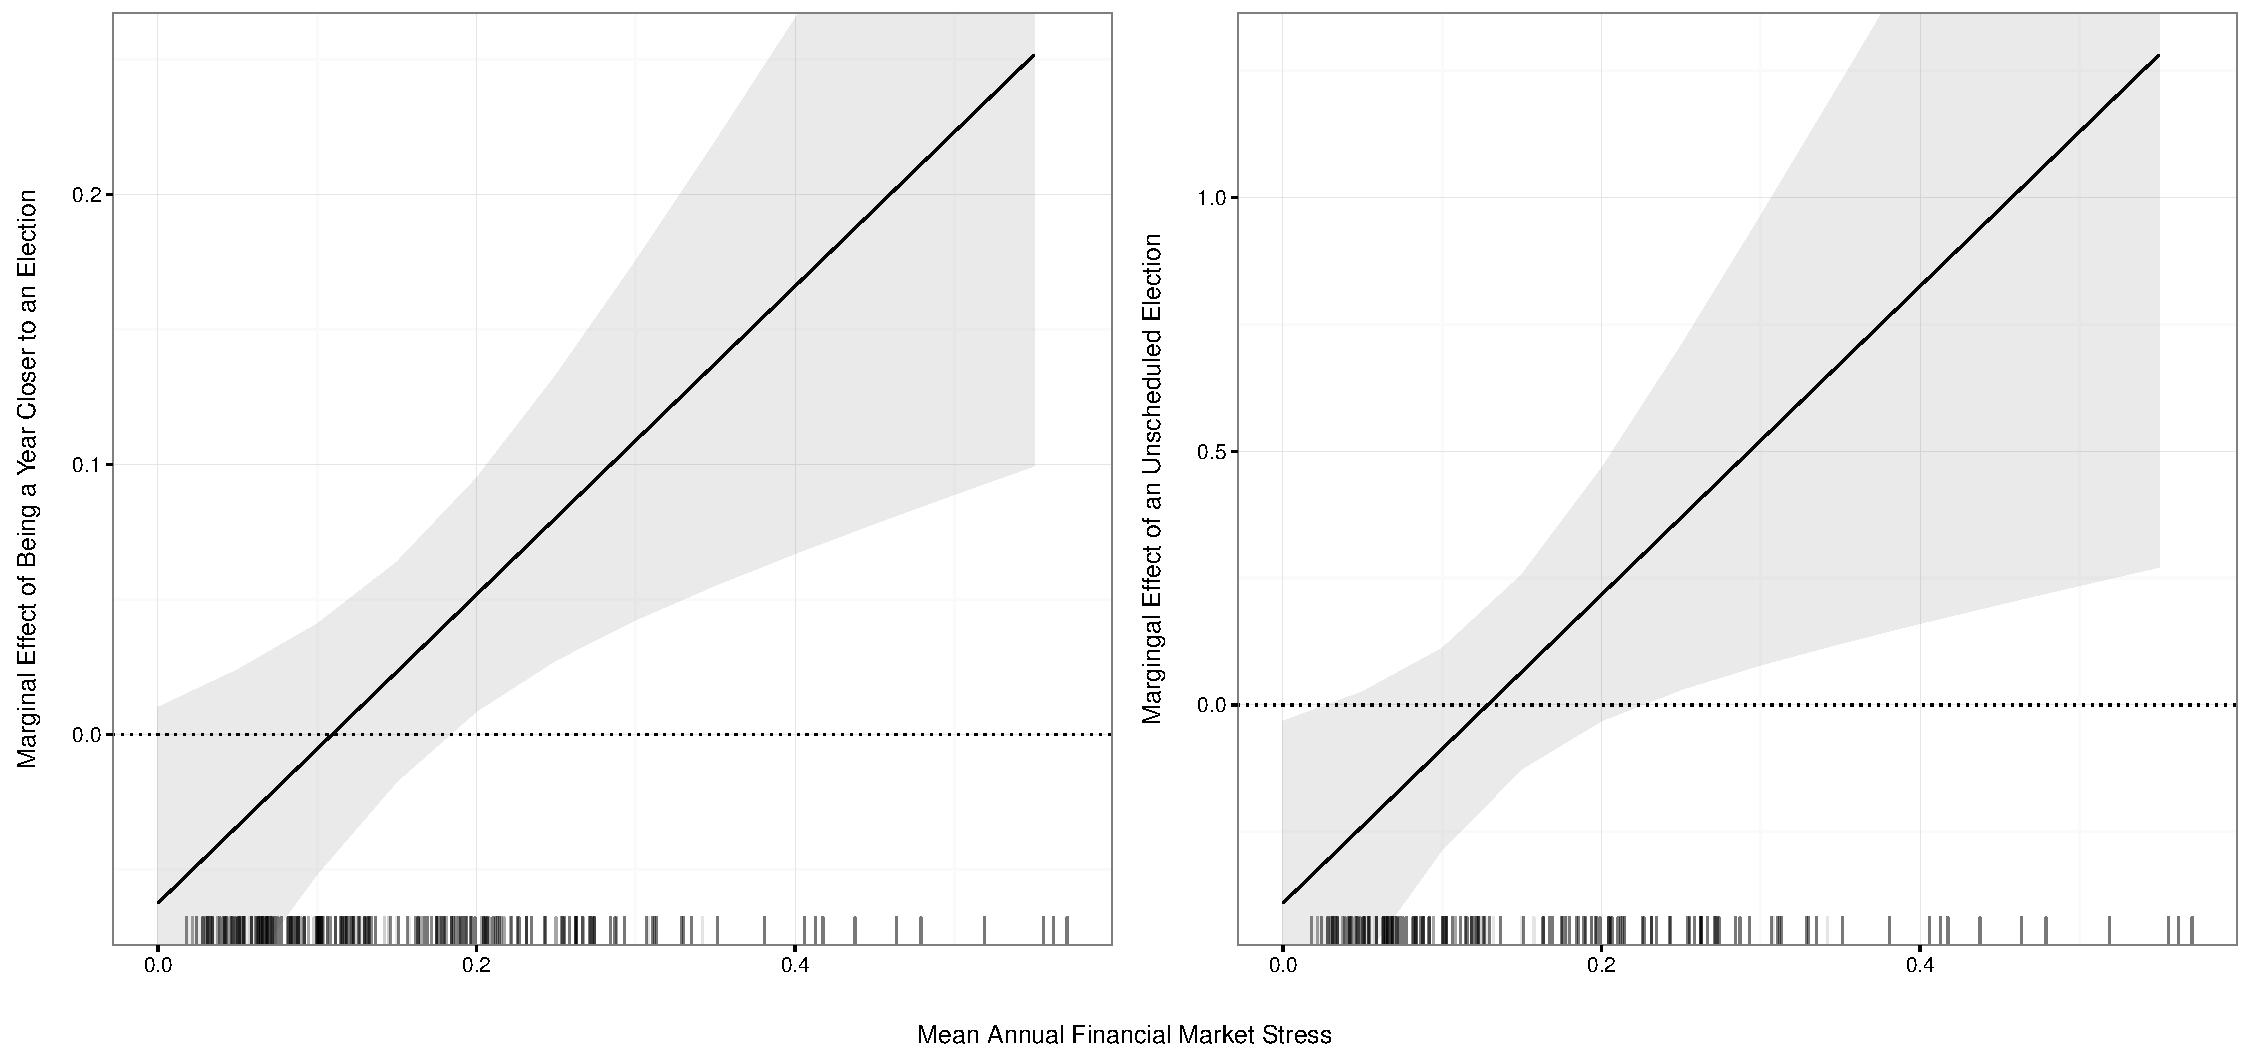
\includegraphics[scale=0.4]{figures/debt_me_nogreece.pdf}
    \end{center}

	{\scriptsize{Shaded area represents 95\% confidence interval.}}

\end{figure}

\begin{figure}[H]
    \caption{Marginal Effects of Eurozone Membership and Being in an EDP at Various Levels of Government Debt and Years to Election on \textbf{Debt} Revisions (sample excluding Greece)}
    \label{me_no_greece_edp_timing}

    \begin{center}
        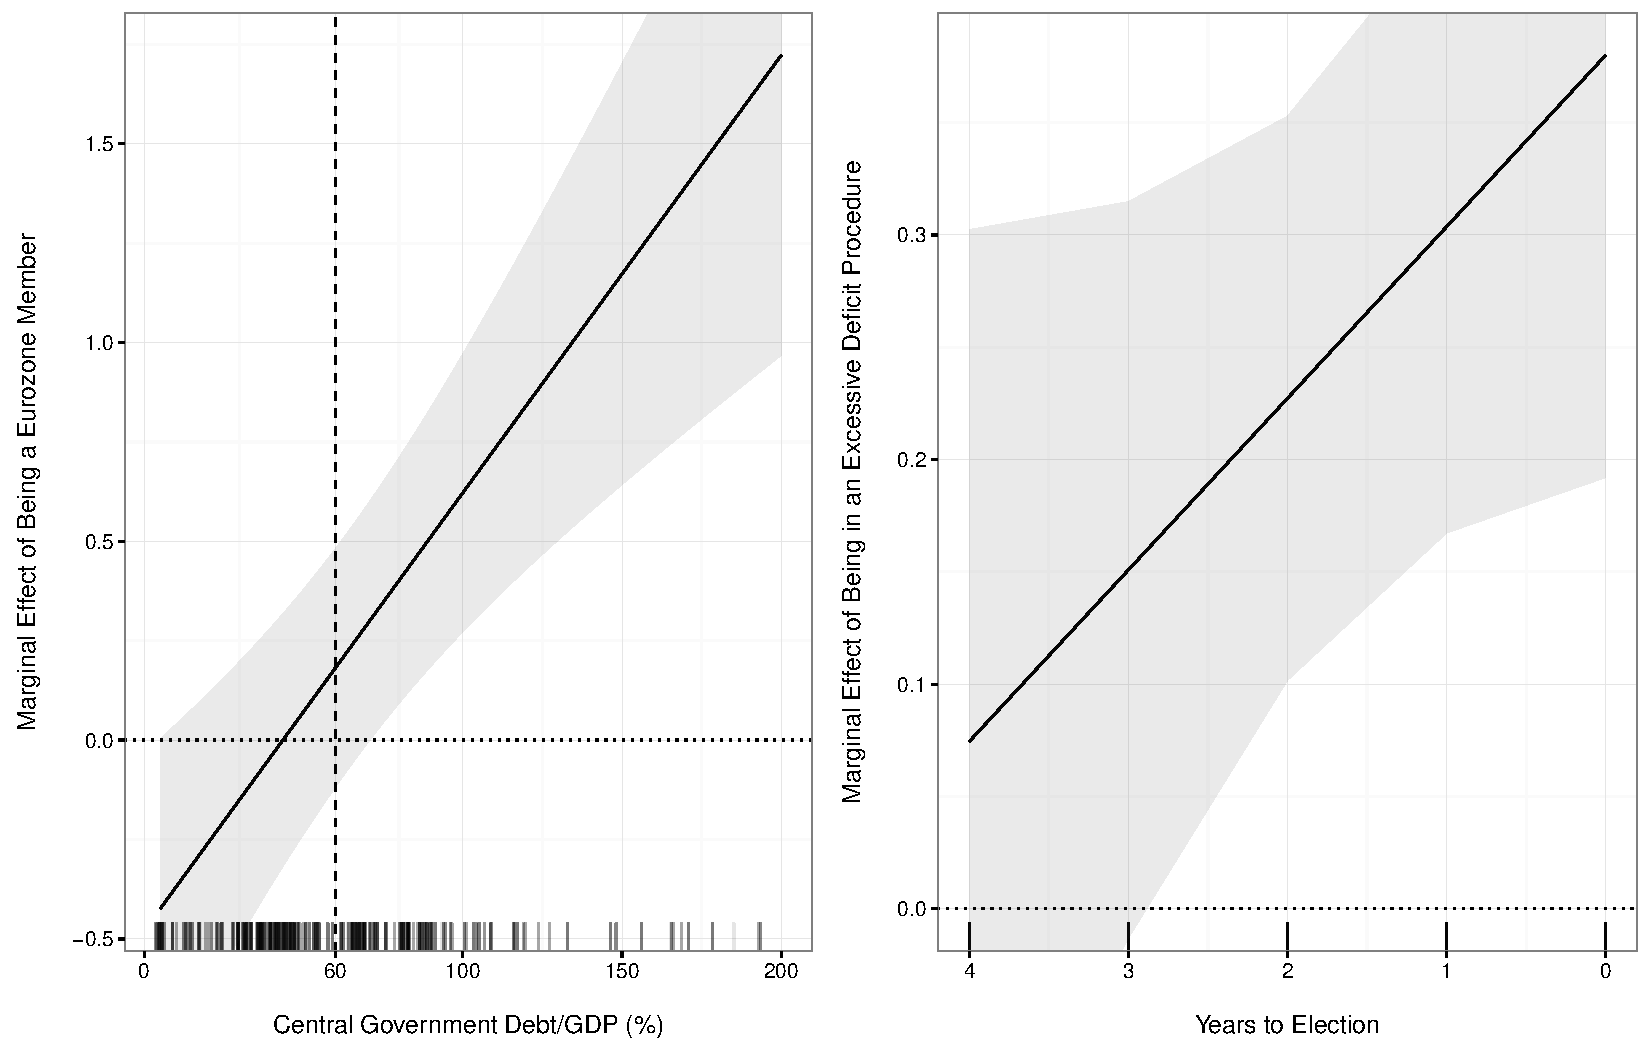
\includegraphics[scale=0.5]{figures/edp_debt_elect_me_nogr.pdf}
    \end{center}

	{\scriptsize{Shaded area represents 95\% confidence interval.}}

\end{figure}

\subsection*{Deficit Revisions}

In addition to debt revisions explored in the main text, we also explored deficit revisions in a similar manner. First we examine deficit revisions descriptively. Figure \ref{median_deficit_revisions} (similar to Figure \ref{median_debt_revisions} in the main text) shows the cumulative Eurostat deficit revisions in our sample under different electoral conditions. The electoral pattern is somewhat less clear for deficit revisions than debt revisions discussed in the main paper. Though the possible effect is in the same theoretical direction as we found in the debt revisions.

In the left-panel of Figure \ref{median_deficit_revisions} years far away from a scheduled election--i.e. three and four years from the election--deficits are generally either not revised or slightly revised upwards such that the government ran a slight surplus relative to the original data. Conversely, data for years closer to an election are revised somewhat downward. In other words, governments spent more relative to their income than they had originally reported. The right-panel of Figure \ref{median_deficit_revisions} indicates that both scheduled and unscheduled election years see larger median downward deficit revisions. There appears to be a small difference between these two types of elections with unscheduled elections having somewhat larger downward revisions by the seventh revision.

\begin{figure}
    \begin{center}
        \caption{Median \textbf{Deficit} Revisions for Data Released Under Various Electoral Conditions}
        \label{median_deficit_revisions}
        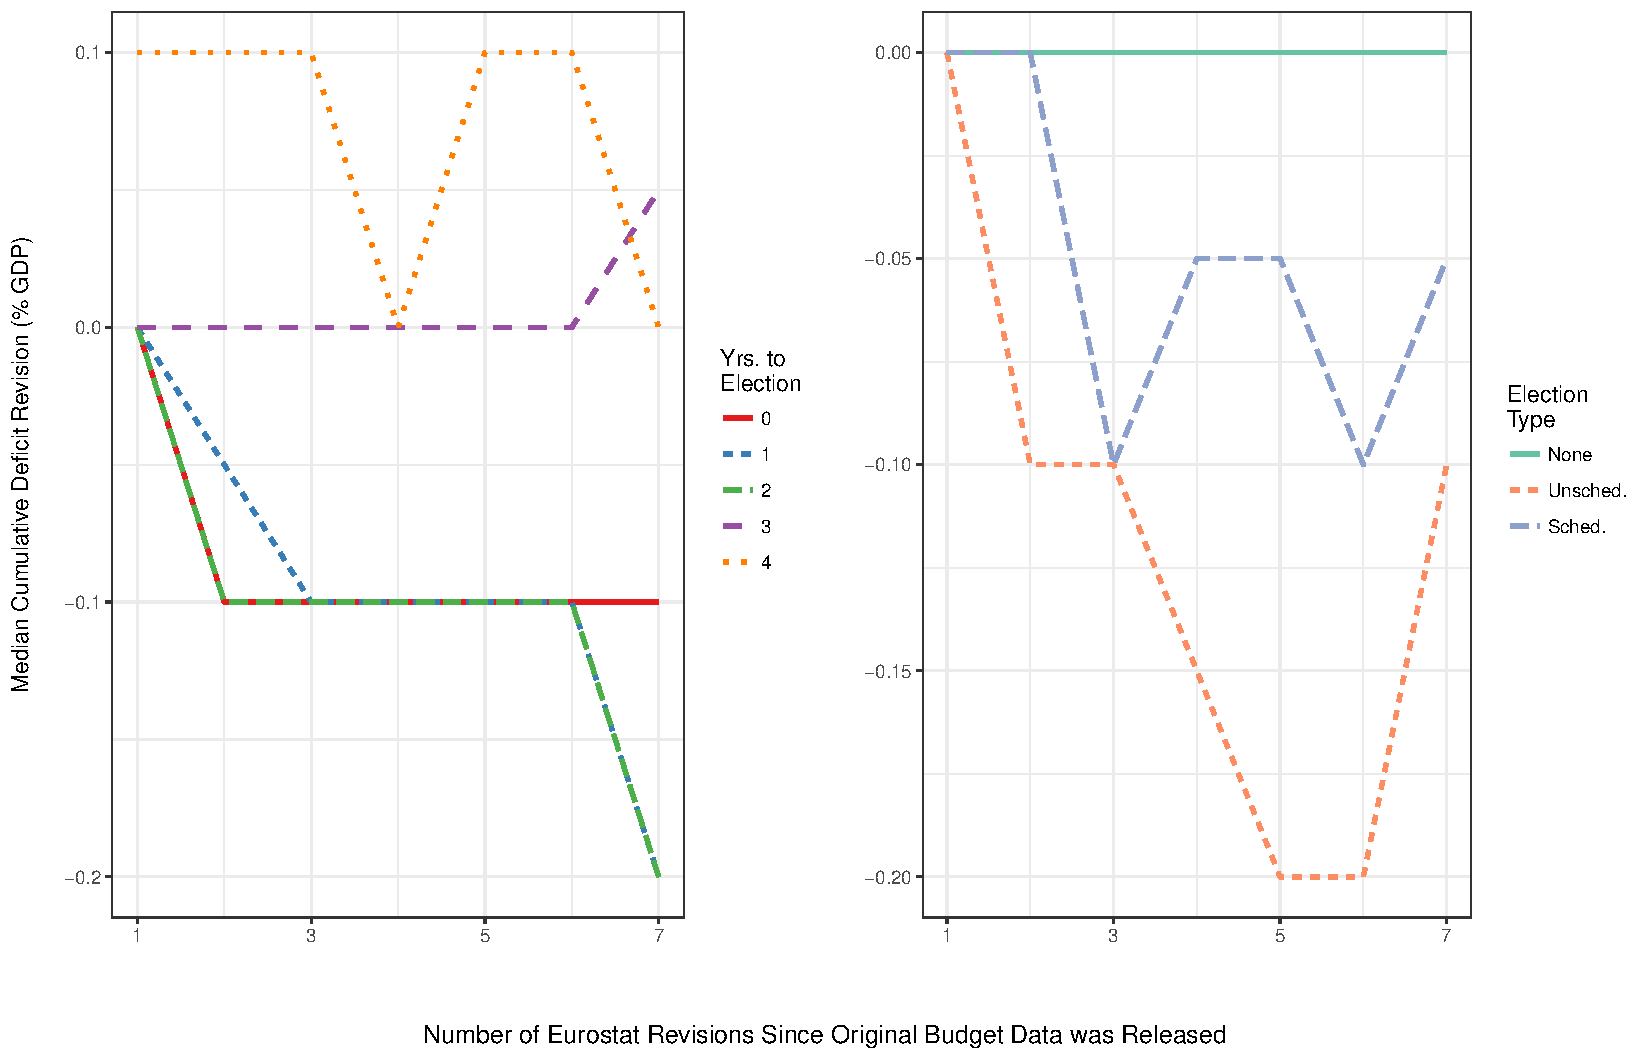
\includegraphics[scale=0.55]{figures/median_deficit_revisions.pdf}
    \end{center}
\end{figure}


We then ran similar models as those found in Table \ref{debt_results} with cumulative deficit revisions as the dependent variable. These results are shown in Table \ref{deficit_results}. We can see that there is no evidence in these models to support hypotheses regarding electoral effects on deficit revisions, including in interaction with financial market stress. This finding is in line with our expectations, as overwhelmingly fiscal rule stretching in response to financial crisis will be on the debt, rather than deficit component of the budget.

\begin{landscape}
    
% Table created by stargazer v.5.2 by Marek Hlavac, Harvard University. E-mail: hlavac at fas.harvard.edu
% Date and time: Thu, Oct 27, 2016 - 13:37:08
\begin{table}[!htbp] \centering 
  \caption{Linear Regression Estimation of Deficit Revisions (Full Sample)} 
  \label{deficit_results} 
\tiny 
\begin{tabular}{@{\extracolsep{5pt}}lcccccccccc} 
\\[-1.8ex]\hline 
\hline \\[-1.8ex] 
 & \multicolumn{10}{c}{\textit{Dependent variable:}} \\ 
\cline{2-11} 
\\[-1.8ex] & \multicolumn{10}{c}{Cumulative Deficit Revisions} \\ 
\\[-1.8ex] & (1) & (2) & (3) & (4) & (5) & (6) & (7) & (8) & (9) & (10)\\ 
\hline \\[-1.8ex] 
 Revised Gen. Gov. Deficit & 0.053$^{***}$ & 0.042$^{*}$ & 0.042$^{*}$ & 0.048$^{***}$ & 0.049$^{***}$ & 0.049$^{***}$ & 0.038$^{**}$ & 0.050$^{***}$ & 0.033$^{**}$ & 0.098$^{**}$ \\ 
  & (0.013) & (0.020) & (0.020) & (0.013) & (0.013) & (0.013) & (0.013) & (0.014) & (0.011) & (0.030) \\ 
  & & & & & & & & & & \\ 
 Euro Member & $-$0.190 & $-$0.180 & $-$0.180 & $-$0.183 & $-$0.192 & $-$0.205 & $-$0.145 & $-$0.179 & $-$0.329 & $-$0.353 \\ 
  & (0.197) & (0.193) & (0.193) & (0.182) & (0.181) & (0.182) & (0.188) & (0.190) & (0.262) & (0.212) \\ 
  & & & & & & & & & & \\ 
 EDP & 0.340$^{**}$ &  &  &  &  &  &  &  &  & 0.346$^{**}$ \\ 
  & (0.104) &  &  &  &  &  &  &  &  & (0.112) \\ 
  & & & & & & & & & & \\ 
 Election Timing &  &  &  & $-$0.014 &  &  &  & $-$0.038 &  &  \\ 
  &  &  &  & (0.027) &  &  &  & (0.124) &  &  \\ 
  & & & & & & & & & & \\ 
 Unscheduled Elect. &  &  &  &  & $-$0.163 & 0.663 &  &  &  & 0.518 \\ 
  &  &  &  &  & (0.153) & (0.640) &  &  &  & (0.661) \\ 
  & & & & & & & & & & \\ 
 Scheduled Elect. &  &  &  &  & 0.115 & $-$0.197 &  &  &  & $-$0.349 \\ 
  &  &  &  &  & (0.090) & (0.369) &  &  &  & (0.427) \\ 
  & & & & & & & & & & \\ 
 Financial Stress &  &  &  & 0.008 & 0.009$^{*}$ & 0.009 &  & 0.007 &  & 0.005 \\ 
  &  &  &  & (0.004) & (0.004) & (0.005) &  & (0.008) &  & (0.006) \\ 
  & & & & & & & & & & \\ 
 Fiscal Transparency &  &  &  &  &  &  & $-$0.001 & $-$0.0003 &  &  \\ 
  &  &  &  &  &  &  & (0.003) & (0.003) &  &  \\ 
  & & & & & & & & & & \\ 
 GDP Growth &  &  &  &  &  &  & $-$0.008 & $-$0.003 &  & $-$0.004 \\ 
  &  &  &  &  &  &  & (0.010) & (0.010) &  & (0.012) \\ 
  & & & & & & & & & & \\ 
 Contracts &  &  &  &  &  &  &  &  & $-$0.669 &  \\ 
  &  &  &  &  &  &  &  &  & (1.999) &  \\ 
  & & & & & & & & & & \\ 
 Debt * Euro &  & $-$0.013 & $-$0.013 &  &  &  &  &  &  & $-$0.042 \\ 
  &  & (0.024) & (0.024) &  &  &  &  &  &  & (0.029) \\ 
  & & & & & & & & & & \\ 
 Elect. Timing * Fin. Stress &  &  &  &  &  & $-$0.017 &  &  &  & $-$0.016 \\ 
  &  &  &  &  &  & (0.013) &  &  &  & (0.013) \\ 
  & & & & & & & & & & \\ 
 Unscheduled Elect. * Fin. Stress &  &  &  &  &  & 0.007 &  &  &  & 0.011 \\ 
  &  &  &  &  &  & (0.008) &  &  &  & (0.009) \\ 
  & & & & & & & & & & \\ 
 Scheduled Elect. * Fin. Stress &  &  &  &  &  &  &  & 0.001 &  &  \\ 
  &  &  &  &  &  &  &  & (0.003) &  &  \\ 
  & & & & & & & & & & \\ 
 Constant & $-$0.322 & $-$0.303 & $-$0.303 & $-$0.654$^{*}$ & $-$0.696$^{*}$ & $-$0.704$^{*}$ & $-$0.265 & $-$0.551 & 0.464 & $-$0.428 \\ 
  & (0.267) & (0.259) & (0.259) & (0.314) & (0.310) & (0.324) & (0.273) & (0.457) & (1.839) & (0.381) \\ 
  & & & & & & & & & & \\ 
\hline \\[-1.8ex] 
Country FE? & Yes & Yes & Yes & Yes & Yes & Yes & Yes & Yes & Yes & Yes \\ 
Observations & 413 & 460 & 460 & 460 & 460 & 460 & 460 & 460 & 423 & 413 \\ 
R$^{2}$ & 0.286 & 0.267 & 0.267 & 0.274 & 0.279 & 0.283 & 0.268 & 0.274 & 0.265 & 0.306 \\ 
Adjusted R$^{2}$ & 0.232 & 0.216 & 0.216 & 0.221 & 0.225 & 0.226 & 0.215 & 0.216 & 0.215 & 0.240 \\ 
\hline 
\hline \\[-1.8ex] 
\textit{Note:}  & \multicolumn{10}{r}{$^{*}$p$<$0.05; $^{**}$p$<$0.01; $^{***}$p$<$0.001} \\ 
\end{tabular} 
\end{table} 

\end{landscape}

\end{document}
